\section{自律校正の原理}
図\ref{fig:校正系}に自律校正を行う装置校正を示す.同じセンサを2つ用意し,変位を与えるレバーを用意する.この時支点からzの位置に校正するセンサBを配置し,nzの位置に基準とするセンサAを配置する.すると基準側の変位は被校正側のn倍となる.
\begin{figure}[htbp]
    \centering %中央揃え
    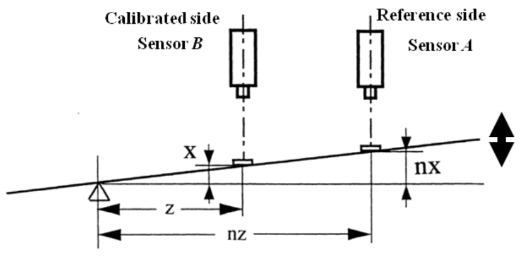
\includegraphics[width=100truemm,clip]{fig/fig_校正系.png}
    \caption{Autonomous calibration device configuration.}
    \label{fig:校正系}
\end{figure}

図\ref{fig:step1}に校正のstep1(n = 2)を示す.まず基準側のセンサAで平均感度から変位$X_{Mea}$を求める.True curveを仮定すると誤差$e_{A0}$は次式で求められる.
\begin{equation}
    e_{A0} = X_{True} - X_{Mea}
\end{equation}
次に$X_{Mea}$の値を用いてセンサBの校正を行う.被校正側の変位は基準側の1/nであるから誤差$e_{B1}$は次式で求められる.ここで変位が基準側の1/nになることから,レバーを動かすことで基準側ではn回の測定を行うことになる.
\begin{equation}
    e_{B1} = \frac{X_{True}}{n} - \frac{X_{Mea}}{n} = \frac{e_{A0}}{n}
    \label{eq:誤差B1}
\end{equation}

\begin{figure}[htbp]
    \centering %中央揃え
    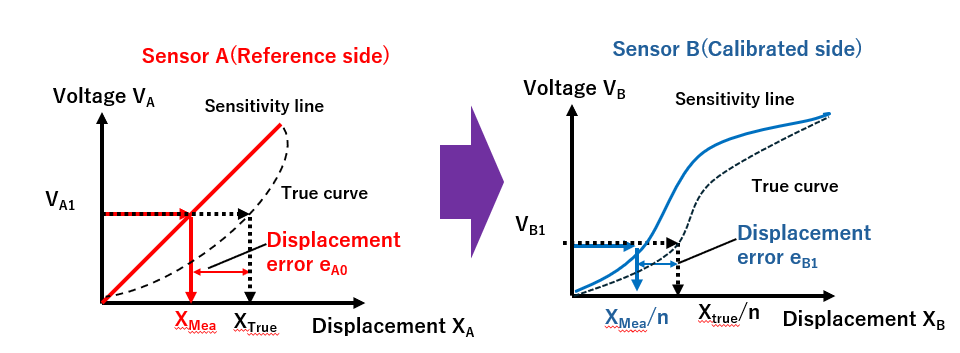
\includegraphics[width=120truemm,clip]{fig/fig_step1.png}
    \caption{Calibration of sensor B by sensor A(step1).}
    \label{fig:step1}
\end{figure}
図\ref{fig:step2}に校正のstep2(n = 3)を示す.センサAとBの位置を入れ替え,センサBを基準側とする.センサBの校正曲線から誤差は式(\ref{eq:誤差B1})で求められる.次にセンサBの$X_{Mea}$を用いて,センサAの校正を行う.誤差$e_{A2}$は次式で求められる.
\begin{equation}
    e_{A2} = \frac{X_{True}}{n} - \frac{X_{Mea}}{n} = \frac{e_{B1}}{n} = \frac{e_{A0}}{n^2}
    \label{eq:誤差A2}
\end{equation}
\begin{figure}[htbp]
    \centering %中央揃え
    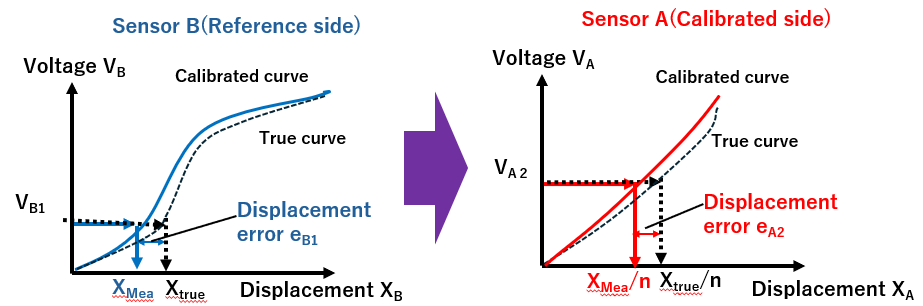
\includegraphics[width=120truemm,clip]{fig/fig_step2.png}
    \caption{Calibration of sensor A by sensor B(step2).}
    \label{fig:step2}
\end{figure}

以上の手順をk回繰り返すと,誤差$e_{Ak-1}$,$e_{Bk}$は次式で求められる.
\begin{equation}
    e_{Ak-1} = \frac{e_{A0}}{n^{k-1}}
    \label{eq:誤差Ak-1}
\end{equation}
\begin{equation}
    e_{Bk} = \frac{e_{A0}}{n^{k}}
    \label{eq:誤差Bk}
\end{equation}
このようにkが大きくするにつれて誤差が小さくなっていることが分かる.これが自律校正の原理である.